Tässä luvussa esitetään tutkimuksen tärkein sisältö ja kokonaisuutena vastaus tutkimuskysymykseen \emph{T1}, eli toistettavissa oleva menetelmä testitapauksien priorisoimiseen.
Priorisointiin vaikuttavat muuttujat luvussa \ref{ch:10_priorisointiin_vaikuttavat_muuttujat} esitetään myös suora vastaus tutkimuskysymykseen \emph{T2}.
Lisäksi painofunktiot \ref{ch:10_painofunktiot_priorisointiin} ja verkon karsiminen \ref{ch:10_verkon_karsiminen} esittää vastaukset tutkimuskysymykseen \emph{T3}.
Testitapauksien muodostaminen verkosta \ref{ch:10_testitapauksien_muodostaminen_verkosta} antaa osittaisen vastauksen myös tutkimuskysymykseen \emph{T4}.

Priorisointia varten esitetään harkintaa käyttäen lähdeaineistosta suodatetut priorisointiin vaikuttavat muuttujat, painofunktio, testitapauksien näkymäperusteinen koostaminen ja painotetun verkon laatiminen.
Lisäksi menetelmää käyttäen tuotetun painotetun verkon sisältämää informaatiota käytetään prioriteeteiltaan tärkeiden polkujen löytämiseen ja testikattavuuden arviointiin.

\section{Priorisointiin vaikuttavat muuttujat} \label{ch:10_priorisointiin_vaikuttavat_muuttujat}

  Näkymä- ja siirtymäperustaiseen priorisointiin vaikuttavat muun muassa seuraavat muuttujat.

  \begin{itemize}
    \item Liiketoiminnallinen arvo
    \item Liiketoiminnallinen visio
    \item Käyttäjäpalaute
    \item Käyttötapauksien määrä näkymässä
    \item Näkymään johtavien siirtymien määrä
    \item Käyttäjän saama arvo
    \item Riski
    \item Projektin muuttumisen volatiliteetti
    \item Kehittämisen kompleksisuus
    \item Vaatimusten taipumus virheellisyyteen
  \end{itemize}

\section{Painofunktiot priorisointiin} \label{ch:10_painofunktiot_priorisointiin}

  Painofunktion yleinen kuvaus verkossa \(G\), solmuille \(V\) ja kaarille \(E\).
  \[\alpha := V(G), E(G) \rightarrow \mathbb{N}\]

  Painofunktio yksittäiselle solmulle \(v\), eli näkymälle.
  \[\alpha(v) = value + vision \pm feedback - volatility - complexity - errorness\]

  Painofunktio yksittäiselle kaarelle \(e\), eli siirtymälle.
  \[\beta(e) = value - volatility - complexity - errorness\]

  Painofunktion polulle \(P\) solmusta \(v_1\) solmuun \(v_2\).
  \[\gamma(P) = \sum_{v \in P} \alpha(v) + \sum_{e \in P} \beta(e)\]

\section{Verkon rakentaminen} \label{ch:10_verkon_rakentaminen}

  % TODO: Esitä esimerkkinäkymät ja relaatiot
  <TODO: Miten verkon solmut ja kaaret poimitaan käyttöliittymästä>

  <TODO: Selitä A-J näkymät, jota varten painomatriisi ja esimerkkigraafi on tehty.
  \begin{itemize}
    \item \textbf{A:} Kirjautumisnäkymä
    \item \textbf{B:} Pelivalikkonäkymä
    \item \textbf{C:} Pelinäkymä
    \item \textbf{D:} Asetusnäkymä
    \item \textbf{E:} Ostonäkymä
    \item \textbf{F:} Ohjenäkymä
    \item \textbf{G:} Tulosnäkymä
    \item \textbf{H:} Onnittelunäkymä
  \end{itemize}

  % TODO: Päivitä painomatriisi vastaamaan esimerkkiä
  <TODO: Esimerkki painomatriisista, jota käytetään priorisoinnin syötteenä>
  \[
    M_G =
    \bordermatrix{
      G & v_a & v_b & v_c & v_d & v_e & v_f & v_g & v_h & v_i & v_j \cr
      v_a & \infty & 1 & 1 & 1 & 1 & 1 & 1 & 1 & 1 & 1 \cr
      v_b & 1 & \infty & 1 & 1 & 1 & 1 & 1 & 1 & 1 & 1 \cr
      v_c & 1 & 1 & \infty & 1 & 1 & 1 & 1 & 1 & 1 & 1 \cr
      v_d & 1 & 1 & 1 & \infty & 1 & 1 & 1 & 1 & 1 & 1 \cr
      v_e & 1 & 1 & 1 & 1 & \infty & 1 & 1 & 1 & 1 & 1 \cr
      v_f & 1 & 1 & 1 & 1 & 1 & \infty & 1 & 1 & 1 & 1 \cr
      v_g & 1 & 1 & 1 & 1 & 1 & 1 & \infty & 1 & 1 & 1 \cr
      v_h & 1 & 1 & 1 & 1 & 1 & 1 & 1 & \infty & 1 & 1 \cr
      v_i & 1 & 1 & 1 & 1 & 1 & 1 & 1 & 1 & \infty & 1 \cr
      v_j & 1 & 1 & 1 & 1 & 1 & 1 & 1 & 1 & 1 & \infty \cr
    }
  \]

  % TODO: Päivitä kuva vastaamaan esimerkkiä
  <TODO: Esimerkki painotetusta verkosta, jota käytetään priorisoinnin syötteenä>
  \begin{figure}[H]
    \centering
    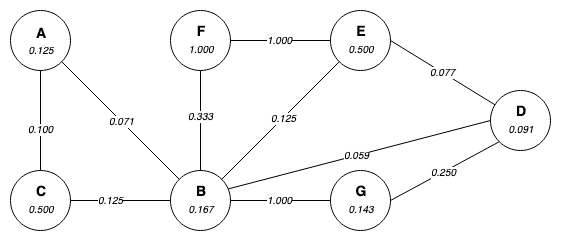
\includegraphics[width=0.8\textwidth]{assets/painotettu-verkko-ennen.png}
    \caption{Esimerkki painotetusta verkosta ennen leikkauksia}
    \label{fig:painotettu-verkko-ennen}
  \end{figure}

\section{Verkon karsiminen} \label{ch:10_verkon_karsiminen}

  Painotetun verkon karsiminen eli leikkaaminen on prioriteeillä painotetun verkon tärkeä ominaisuus.
  Verkkoteorian soveltaminen prioriteettien avulla painotettuun verkkoon on erityisen hyödyllistä, kun verkon kaarissa korkea paino tarkoittaa suurta prioriteettia.
  Tällaisessa tapauksessa on mahdollista soveltaa lyhimmän polun ongelman ratkaisemiseen kehitettyjä algoritmeja, jolloin ne toimivat etsien alhaisimman prioriteetin polkuja.
  Lyhimmän polun etsimiseen on tarkoituksenmukaista valita aina aloitus ja lopetuspisteet, joiden välille lyhin polku verkossa voidaan etsiä.
  Prioriteetein painotetun verkon karsimistarkoitukseen olisi järkevää valita sellaiset aloitus- ja lopetuspisteet, joiden välillä ei näyttäisi olevan korkean prioriteetin solmuja.
  Voidaan kuitenkin menetellä myös siten, että valitaan aloitus- ja lopetuspisteeksi sellaiset solmut, jotka ovat painoltaan verkon alhaisimmat \(v_1 = min(V)\) ja \(v_2 = min(V \setminus \{v_1\})\) ja esimerkiksi verrata niiden lyhimmän polun kokonaisprioriteettia muuhun verkkoon.

  \begin{itemize}
    \item Pienimmän prioriteetin solmuparin etsiminen, eli \(v_1 = min\{ \alpha(V) \}\) ja \(v_2 = min\{\alpha( V \setminus \{v_1\} \}\).
    \item Dijkstran algoritmin käyttö lyhimmän (prioriteetiltaan pienimmän) polun löytämiseen, eli \(s = min( \gamma(P) ), P \in G\).
    \item Leikkauksien tekeminen ja toistaminen \(n\)-kertaa.
    \item Poistetaan yhden yksittäiseen solmuun johtavat sillat, jossa \(\alpha(v) < aivan liian alhainen \).
    \item Poistetaan kaikki yksittäiset eristetyt solmut, eli asteluku on nolla \(d_G(X) = 0\).
    \item Poistetaan Dijkstran lyhimmän polun kaaret, jossa \(\beta(e) < liian alhainen \).
  \end{itemize}

  % TODO: Päivitä kuva vastaamaan esimerkkiä
  \begin{figure}[H]
    \centering
    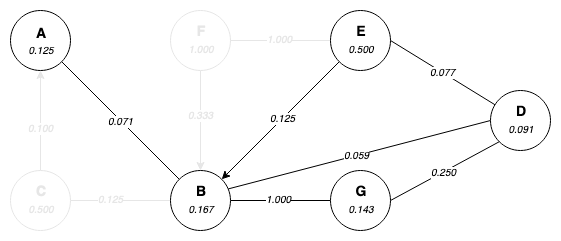
\includegraphics[width=0.8\textwidth]{assets/painotettu-verkko-jalkeen.png}
    \caption{Esimerkki painotetusta verkosta leikkauksien jälkeen}
    \label{fig:painotettu-verkko-jalkeen}
  \end{figure}

\section{Verkon ja testitapauksien yhteys} \label{ch:10_verkon_ja_testitapauksien_yhteys}

  Ennen testitapauksien suunnittelua tehtävä priorisointi kuvainnollistaa käyttöliittymän näkymiä, niiden osanäkymiä ja niiden välisiä siirtymiä.
  Tällaisesta painotetusta verkosta saadaan priorisoitua näkymät ja siirtymät, mutta lopulliset testitapauksien prioriteetit ovat testitapaukseen kuuluvien näkymien tai siirtymien prioriteetteja.
  Tämä tarkoittaa käytännössä sitä, että kun näkymät ja siirtymät on priorisoitu, on esimerkiksi yhden yksittäisen tarkasteltavana olevan näkymän toiminnoilla sama keskenään prioriteetti.
